\chapter{Costruiamo una teoria che descriva un plasma}

\begin{approfondimento}{Elemento fluido}
	\begin{multicols}{2}
		Possiamo basare la nostra descrizione del plasma su qualcosa di simile a quel che è l'elemento fluido in fluidodinamica.
		
		L'elemento fluido è un concetto teorico, una regione cubica di lato $\ell$ in un più grande sistema di lunghezza caratteristica $L\gg\ell$, tale che la distanza delle particelle all'interno dell'elemento sia $d\ll\ell$.
		
		Per questo l'elemento fluido è da considerarsi come un punto $\vec{x}=(x, y, z)$ e questo ci permette di descrivere il sistema con proprietà intensive (pressione, densità, velocità) per singolo elemento.
		
		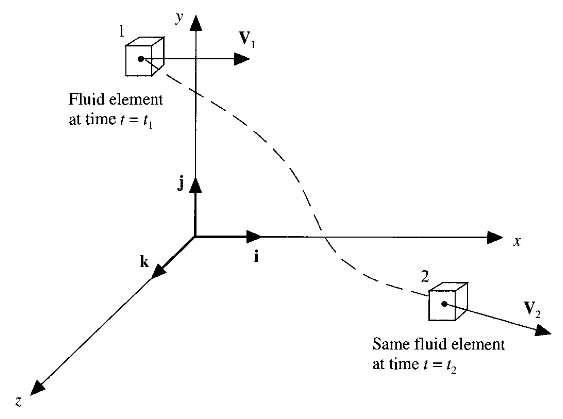
\includegraphics[width=7cm]{immagini/A-23.png}
	\end{multicols}
	Le grandezze definite per il cubetto (grandezze termodinamiche) diventano campi continui: ad esempio $\rho(\vec x)$, $p(\vec x)$, ... 
	
	Il cubetto $\Delta V$, detto \textit{elemento fluido}, ha la caratteristica che il tempo con cui una molecola ne fuoriesce è molto maggiore del tempo caratteristico di evoluzione del sistema (dato l'altissimo numero di collisioni/ rateo di collisioni).
	
	La descrizione è sensata per un fluido in cui $\displaystyle\frac{\nu_c}{\omega_D}\rightarrow +\infty$ perché le particelle collidono così spesso da rimanere all'interno dell'elemento mentre esso si muove, permettendoci di trattare l'e.f. come una "super-particella" di massa $mn\Delta V$ e velocità $\vec{u}$. 
	
	Nei plasmi, generalmente rarefatti e ad alta temperatura, le collisioni sono poche (ad esempio un protone del vento solare tipicamente ha al massimo una interazione in 1~U.A.). 
	Le particelle in un cubetto non sono quindi le stesse a tempi successivi. Tuttavia, è possibile individuare regimi in cui il plasma si comporta come un fluido: si ottengono le stesse equazioni, ma senza poggiarsi sugli stessi pilastri teorici della fluidodinamica.  
	
	Come può quindi essere valido per un plasma in cui $\displaystyle\frac{\nu_c}{\omega_D}\rightarrow 0$? perché i la presenza di campi esterni genererà movimento delle particelle con un certo raggio di girazione, sarà questo e non le collisioni a definire la dimensione $\ell^3$ dell'elemento fluido.
\end{approfondimento}

\begin{approfondimento}{Derivata lagrangiana}
	Nel seguito apparirà più volte la derivata lagrangiana, anche detta "materiale" o "collettiva", operatore ricorrente della meccanica del continuo e della fluidodinamica:
	\[ \frac{D}{Dt}[\ \textit{f}\ ]\ \ =\ \ \frac{\partial \textit{f}}{\partial t}\ +\ \vec{u}\cdot\vec{\nabla} \textit{f}\ \ \ , \]
	dove $\vec{u}\cdot\vec{\nabla}$ è il termine \underline{convettivo} che tiene conto di come il campo \textit{f} vari non nel tempo ma come effetto del flusso del campo stesso.
	
	\noindent Più in particolare, la derivata lagrangiana della velocità, $\frac{D}{Dt} \vec{u} = \frac{\partial}{\partial t} \vec{u} + \vec{u}\cdot\vec{\nabla} \vec{u}$ viene chiamata accelerazione idrodinamica ed è frequente in fluidodinamica, ma incontreremo molte derivate lagrangiane di altre quantità.
\end{approfondimento}
\vspace{0.5cm}
Andiamo a definire nelle prossime sezioni le equazioni che saranno il pilastro della nostra teoria fluida, legate ad una visione euleriana della teoria dei plasmi che andremo a costruire in questo capitolo, nella quale descriveremo dei campi quali la densità $\rho(\vec{x}, t)$, la velocità $\vec{v}(\vec x, t)$, la pressione $p(\vec{x}, t)$, la densità di carica $\rho_q(\vec{x}, t)$, la corrente $\vec{J}(\vec{x}, t)$ oltre che chiaramente $\vec{E}(\vec{x}, t)$ e $\vec{B}(\vec{x}, t)$.




\subsection{Equazione di continuità}
Prima equazione della fluidodinamica, anche detta equazione di continuità della massa, è valida trascurando gli effetti di ricombinazione e ionizzazione che alterano il numero di ioni/elettroni nella popolazione, si ricava facilmente con un approccio euleriano e usando il teorema della divergenza: 
\[\int_A\rho\vec v \hspace{1mm} d\vec A=-\frac{\partial}{\partial t}\int_V\rho dV\ \ \ \ \ \ \Rightarrow\ \ \ \ \ \
\int_V\vec\nabla(\rho \vec v)dV=\int_V-\frac{\partial\rho}{\partial t} dV\]

\begin{equation}
	\label{fluid-continuità}
	\Rightarrow \ \ \ \ \ \boxed{
		\frac{d\rho}{dt} + \vec{\nabla} \cdot (\rho \vec u) = 0}\ \ \ \  ,
\end{equation}


dove $\displaystyle \frac{\partial \rho}{\partial t}$ è la variazione locale della densità nel tempo, che non è altro che equivalente al flusso di materia che entra ed esce dall'elemento fluido, il flusso di massa $-\vec{\nabla}\cdot(\rho \vec{u})$. 

Riconosciamo, sviluppando $\vec{\nabla} \cdot (\rho \vec u) = (\vec{u}\cdot\vec\nabla)\rho + \rho \vec\nabla\cdot\vec{u}$, che due termini possono essere accorpati per riscrivere la formula usando una derivata materiale:
\[ \Big(\frac{d\rho}{dt} + (\vec{u}\cdot\vec\nabla)\rho\Big) + \rho \vec\nabla\cdot\vec{u}\ =\ \frac{D}{Dt}\rho + \rho\vec\nabla\cdot\vec{u}\ =\ 0\ \ \ \ . \]

Interpretazione: un volumetto di fluido può cambiare densità solo comprimendosi o espandendosi. 
Nel limite di incomprimibilità si impone $\vec\nabla\cdot\vec{u}=0$ e rimane solamente $\frac{D\rho}{Dt}=0$; questo limine è utile quando si studiano fenomeni senza compressione (es. onde trasversali EM, onde di Alfvén), fenomeni longitudinali come le onde magnetosonore, invece, prevedono compressione e richiedono di non imporre la incomprimibilità.

\subsection{Equazioni del moto (tre componenti)}
Da uno studio della lagrangiana e quindi delle forze che agiscono sull'elemento, si ottiene quella che in fluidodinamica è l'equazione idrodinamica. Consideriamo solamente le forze interne all'elemento fluido perché tendenzialmente in un fluido la pressione è isotropa e quindi all'esterno è tutto compensato. 
\[\vec F=-\int Pd\vec A=-\int \vec \nabla PdV\] sfruttando il punto di vista lagrangiano seguo l'elemento che accelera. Otteniamo così la nostra equazione del moto simil $\vec F = m\vec a$:
\[\rho\frac {D}{Dt}\vec u=-\vec \nabla P\] \
\[ \rho \left[ \frac{\partial \vec u}{\partial t} + (\vec u \cdot \vec \nabla)\vec u \right] = -\nabla P + \text{grav} + \text{col} + \dots  \ \ \ \ .\]
\noindent Oltre la pressione in genere si usa almeno anche un termine gravitazionale:

\begin{equation}\label{fluid-eq-moto}
	\boxed{
		\rho\ \frac{D}{D t} \vec u  = -\vec\nabla p + \rho \vec g +  \vec f} \ \ \ \ .
\end{equation}

Aggiungiamo un termine $\vec f$ perché ci aspettiamo che per i plasmi ci siano anche forze elettromagnetiche che in questa prima forma puramente fluidodinamica non esplicitiamo (cfr. equazioni di Eulero).

\subsection{Equazione di stato}
Noi vorremmo risolvere il sistema di equazioni che stiamo costruendo per 5 variabili ($\vec u$, p, $\rho$), quindi, le quattro equazioni appena introdotte non bastano, il sistema necessità di una chiusura, qui interviene l'equazione di stato della pressione in funzione della densità:
\begin{equation}
	\label{polytropic}
	P(\rho),\, \text{ad esempio una politropica tipica dei fluidi:} \quad P = c \rho^\gamma
\end{equation}
Alla fine ci sono tante variabili (3 componenti della velocità + densità + pressione = 5 variabili) quante equazioni (una di conservazione della massa, tre equazioni del moto, la politropica): il sistema è chiuso. 


\subsection{Evoluzione dell'elemento fluido} 
In fluidodinamica si studia l'evoluzione dell'\textit{elemento fluido}. Ho un fluido e nei vari punti la velocità varia  soprattutto per la condizioe di cut0 dei bordi. (nei casi si fluido incomprimibile come l'acqua allora è inevitabile che si formino dei vortici)\\L'evoluzione dell'elemento fluido  può essere descritta in due modi:
\begin{itemize}
	\item \textbf{Approccio \underline{lagrangiano}}: Si segue il cubetto nel tempo.  "Metto una paperella nel fiume e vedo dove va a finire", o meglio, scelgo un elemento fluido e vedo dove va a finire. In un momento iniziale $t_0$ mi trovo in $x_0=x(t_0)$ e in un momento successivo mi troverò in un altro punto. posso definire la velocità lagrangiana che è la velocità $\vec v(\vec x(t),t)$ del mio elemento fluido. Nei momenti successivi l'elemento fluido si sarà spostato di $\vec \xi (t)=\int_{t_0}^t\vec v(\vec x(t'),t')dt'$ e si troverà nel punto \[\vec x(t)=\vec x_0+\vec \xi(t)\ \] ;
	\item \textbf{Approccio \underline{euleriano}}: si osservano quantità fisiche in un punto fisso dello spazio come una stazione meteo. Fisso un sistema di riferimento e guardo cosa viene e cosa va.  definisco la velocità del fluido rispetto al mio sistema di riferimento, $\vec u(\vec x,t)$ con $\vec x $ che è un punto fissato. inizialmente in $x$ ho un elemento fluido che se ne va e al suo posto ci sarà un nuovo elemento fluido.
\end{itemize}



Per precisione: chiamiamo $t_E$ e $t_L$ i tempi nei due approcci (anche se sono uguali). Le velocità si indicano $\vec u$ (euleriana) e $\vec v$ (lagrangiana).  

In approccio lagrangiano:
\[
\vec x(t_L) = \vec x_0 + \vec \xi(\vec x_0,t_L), 
\qquad 
\vec v = \frac{d\vec \xi}{dt}
\]
\medskip
Poiché $\displaystyle\frac{\partial \vec x}{\partial t} = \frac{\partial \vec \xi}{\partial t} \quad \Rightarrow \quad \vec v = \vec u$

\medskip
A proposito di questi due approcci: torniamo a $\frac{D}{Dt}n+ (\vec u\cdot\vec \nabla)n=0$, la derivata lagrangiana della densità ci fa vedere che seguendo l'elemento fluido l'unica cosa che può far variare la densità è una compressione (o rarefacimento) del mio fluido. \\Fare la derivata euleriana equivale alla derivata lagrangiana a meno di un termine correttivo che tiene conto della direzione in cui va il mio fluido. 
\medskip

Per chiudere il sistema in termodinamica si assume spesso isotropia ($P\propto T$)  (tensore degli stress diagonale). Nei plasmi l'isotropia non vale, perché i campi magnetici introducono direzioni privilegiate: parallela al campo (particelle libere) e ortogonale (particelle bloccate). Nonostante la mancanza di equazione di stato, isotropia e collisioni, la MHD (magnetoidrodinamica) funziona in molte condizioni.
\\IN particolare nei plasmi si ha anisotropia per la pressione $P_{\parallel\vec B}\neq P_{\perp\vec B}$, i satelliti nel plasma spaziale misurano una distribuzione maxwelliana solamente sul piano $\perp \vec B$.


\subsection{Ruolo delle collisioni nella diffusione del calore}

Controintuitivamente, molte collisioni riducono la diffusione termica (es. gas perfetto). 

Consideriamo un volumetto V, all'istante t=0 avrà una certa energia interna e flusso di calore dati da:
\[ U\ =\ \rho\, c_v\, T \ \ \ \ ,\]
\[ \vec{q} = -k \ \vec\nabla T\ \ \ \ ,\]
dove $\vec{q}$ è la densità di corrente termica e $k$ la conducibilità. 

L'energia interna varia a seconda: dello scambio di calore, della compressione o dal calore generato internamente:
\[
\frac{\partial}{\partial t}\int U \, dV = -\int (\vec q \cdot \hat n)\, dS \ \ \ \ .
\]
Applicando il teorema della divergenza:
\[\int_{\partial V} (\vec q \cdot \hat n)\, dS\ =\ \int \vec\nabla \cdot \vec q\, dV \quad \quad \Rightarrow \quad\quad \frac{\partial U}{\partial t}\ =\ -\vec\nabla \cdot \vec q = -k\, \nabla^2 T \ \ \ \ .\]

Se non c’è flusso di massa $\Rightarrow d\rho/dt = 0$, quindi:
\[
\frac{\partial U}{\partial t}\ =\ \rho\, c_v\, \frac{dT}{dt} 
\quad\quad \Rightarrow \quad\quad 
\frac{dT}{dt}\ =\ -D\, \nabla^2\, T \ \ \ ,
\]

avendo definito la \underline{diffusività} $\boxed{D = k\, /\, \rho\, c_v}$, che ha dimensioni $[D]=m^2 s^{-1}$ quindi dimensionalmente è tale che $D/L\, \sim\, 1/\tau$, cioè:
\[
D\ \sim \ \lambda_{mfp}^2\, \nu_c\ =\ \frac{v_{th}^2}{\nu_c}\ \ \ \ ,
\]

dove $\boxed{v_{th}\sim\lambda_{mfp}\ \nu_c}$ è la \underline{velocità termica}, $\lambda_{mfp}$ il \underline{libero cammino medio} e $\nu_c$ la \underline{frequenza collisionale}.  
\[\nu_c\to\infty\implies D\to 0\]

Molte collisioni $\Rightarrow$ diffusione lenta di energia $\implies $ comportamento adiabatico $\implies $ ho una relazione tra densità e pressione (equazione di stato politropica). Non confondere collisioni (viscosità) e trasporto di calore.  

\subsubsection{Entropia}
Nei plasmi, se la frequenza collisionale va all'infinito, $\nu_c\rightarrow \infty$ (cioè siamo adiabatici) vale:
\[ \frac{dS}{dt}\ =\ 0 \]
\[ \frac{\partial S}{\partial t}\ +\ (\vec u\cdot \nabla)\, S\ =\ 0 \]

\subsubsection{Entalpia} 
Riprendiamo la definizione di Entalpia $W$dalla termodinamica, le collisioni nei fluidi ci impongono entropia costante nell'elemento fluido (consideriamo $V$ il volume specifico). \\Il giochino adesso è esprimere l'equazione del moto fluida eq.\ref{fluid-eq-moto} (trascurando il campo gravitazionale e altre forze) in termini dell'entalpia:
\[dW\,=\,T\cancelto{0}{dS}\,+\,VdP\,=\,VdP\quad \implies\quad \rho\, \vec \nabla\, W\,=\,\vec \nabla\, P\] 
\[\partial _t\vec u\,+\,(\vec u\, \cdot\,\vec \nabla)\vec u\ =\-\vec \nabla\, W\]

\begin{approfondimento}{vorticità}
	Definiamo la vorticità come il rotore del campo di velocità \[\vec w=\vec \nabla\times\vec u \hspace{1cm}w_i=\epsilon_{ijk}\partial_ju_k\] Le linee di campo della vorticità sono dette linee di vorticità. Le linee di vorticità possono essere trasportate e spiegazzate ma non possono venire spezzate e riconnesse. (non bisogna confondere le linee di vorticità con le streamline che sono le linee tangenti al campo di velocità punto per punto) 
\end{approfondimento}

Facendo il rotore dell'equazione dinamica espressa in termini dell'entalpia possiamo trovare la vorticità. Allo stesso tempo possiamo utilizzare una formula del calcolo vettoriale per scrivere la derivata materiale come un rotore più un gradiente. Usiamo anche che per campo scalare $\phi $ (come $W$ e come $|u|^2$) vale $\nabla\times\nabla\phi=0$. 

\[\frac{\partial \vec w}{\partial t} =-\nabla \times \left[ \vec u\times \vec w \right]\]

Quest'equazione descrive l'evoluzione della vorticità.


%
%
%
\subsection{Plasmi e regime fluido, come trattarli} 

Abbiamo introdotto alcune quantità e ragionamenti dalla fluidodinamica, fin'ora non abbiamo però sviluppato un vero modello ad un fluido, per come abbiamo svolto tutto fin'ora sarebbe più opportuno riconoscere che vi siano \underline{due fluidi}, uno per ciascuna specie (il modello a singolo fluido sarà la termodinamica).

Andiamo a vedere tramite linearizzazione, quindi trattando le equazioni viste fin'ora perturbativamente, quali comportamenti del plasma riusciamo già a far emergere con questo primo modello di plasma.

\subsubsection{Linearizzazione delle equazioni} 

Scriviamo le variabili come valore medio più una piccola perturbazione:
\[
\rho = \rho_0 + \delta\rho, \qquad 
\vec u = \vec u_0 + \delta \vec u, \qquad
P = P_0 + \delta P
\]

Una perturbazione è da considerarsi 'piccola' quando $\delta \rho \, / \,\rho \ll 1$ ed i prodotti di termini 'di primo ordine' vengono trascurati: $\delta \rho \, \delta \vec u \ll \rho \vec u$. 
Non vengono semplificati i prodotti tra ordine zero e ordine uno, come si vede di seguito:

\[
(\rho_0 + \delta \rho)(\rho_0 + \delta \rho) 
= \rho_0^2 + 2\rho_0 \delta \rho + \cancelto{0}{(\delta \rho)^2}
\]


\subsubsection{Ancora sulla linearizzazione: il comportamento ondulatorio} 

In generale, stiamo considerando di ogni grandezza, il valore medio e una perturbazione, \[ \text{valore medio:}\ \ \ \ \  x_0\, =\, \frac{1}{V}\int x dV,\hspace{2cm} \text{perturbazione:}\ \ \ \delta x\,\ll\, x_0\]

Quindi scrivendolo per ciascuna grandezza: $\quad \rho = \rho_0 + \delta \rho; \quad \vec u = \vec u_0 + \delta \vec u; \quad p = p_0 + \delta p\ \ .$

\vspace{0.4cm}

Andiamo a linearizzare l'equazione di continuità della massa, assumendo $\rho_0 = cost.$ e, come condizione di equilibrio, $\vec u_0 = 0$ :

\[\displaystyle \frac{\partial}{\partial t} (\rho_0 + \delta\rho)\, +\, \vec\nabla\cdot (\cancelto{=0}{\rho_0\vec u_0}\, +\, \cancelto{=0}{\delta\rho\vec{u_0}}\, +\, \rho_0\vec{\delta u}\, +\, \cancelto{\sim 0}{\delta \rho \vec{\delta u})}\ =\ 0 \ \ \ \ ,\]

il termine all'ordine zero è banalmente nullo, d'altro canto il termine di ordine 2 è trascurabile e rimane il termine di ordine 1:

\[\partial_t (\delta \rho)+\vec \nabla\cdot (\rho_0\vec{\delta u})=0\ \ \ \ \ \ \ \ \ \ \Rightarrow \ \ \ \ \ \
\text{In 1D:}\ \ \  \boxed{\displaystyle\frac{\partial \delta \rho}{\partial t} + \rho_0 \frac{\partial \delta u}{\partial x}\ =\ 0}\ \ \ \ .\]

\vspace{0.5cm}

Prendiamo invece dall'equazione del moto, trascurando le collisioni ed il termine gravitazionale, andiamo a linearizzare l'equazione tenendo i termini di ordine più basso, ponendo $\vec u_0 = 0$, $\partial_t u_0 = 0$ e sottraendo la forma di equilibrio $\rho_0 D_t u_0 = -\vec \nabla P_0$:

\[ (\rho_0 + \delta \rho ) \left[ \frac{\partial}{\partial t}(\cancel{u_0}+\delta u) + [(\cancel{u_0} + \delta u)\cdot \vec \nabla] (u_0 + \delta u) \right] \ =\ -\ \vec \nabla \left( P_0 + \delta P \right)\]

\[\Rightarrow \ \ \ \ \boxed{\ \frac{\partial}{\partial t} (\delta u)\ =\ -\ \frac{1}{\rho_0}\frac{\partial}{\partial x}\delta P\ }\]

\vspace{0.5cm}
Per chiudere il sistema di equazioni utilizziamo l'\textbf{equazione di stato politropica}: $\boxed{P = c\rho^\gamma}$, così che usando $\nabla (\delta P)=c\gamma \rho_0^{\gamma-1}\nabla (\delta \rho)$ (derivante dallo sviluppo binomiale) si possa esprimere il termine destro come $\displaystyle \frac{\partial \delta P}{\partial x} = \gamma \frac{P_0}{\rho_0} \frac{\partial (\delta \rho)}{\partial x}$ .

Definita $c_s^2 = \gamma \displaystyle \frac{P_0}{\rho_0}$ la \textbf{velocità del suono}, possiamo ottenere infine l'\underline{equazione del moto linearizzata}: $\displaystyle \rho_0 \frac{\partial}{\partial t} (\delta u)= c_s^2 \frac{\partial }{\partial x} (\delta \rho)$. 

Abbiamo costruito quindi un modellino fluido in una dimensione costituito dalle equazioni appena presentate ed evidenziate:
\[ \begin{cases}
	\frac{\partial }{\partial t} (\delta \rho)\ =\ \rho_0 \frac{\partial}{\partial x} (\delta u)\ ,\\
	\frac{\partial }{\partial t} (\delta u)\ =\ - \frac{1}{\rho_0}\frac{\partial}{\partial x} (\delta P)\ ,\\
	\delta P = c_s^2 \delta \rho
\end{cases} \]

Inseriamo la terza equazione nella seconda come fatto poco sopra per ottenere l'equazione del moto linearizzata e la deriviamo per $\partial_x$, mentre si deriva l'eq. di continuità nel tempo $\partial_t$ , si vede comparire in entrambe il termine $\displaystyle \frac{\partial^2 u}{\partial x \partial t}$, che isoliamo per ottenere l'uguaglianza:
\[ \frac{\partial^2}{\partial t^2} (\delta \rho)\ =\ c_s^2\ \frac{\partial^2}{\partial x^2} (\delta \rho)\]
Il risultato ci consola, perché vuol dire che le perturbazioni di pressione all'interno del plasma così modellizzato si propagano come un'onda di velocità caratteristica $c_s$. Fornita una piccola perturbazione di densità o pressione, la loro variazione genera un gradiente che accelera il fluido secondo l'equazione del moto, il fluido muovendosi modifica ancora la densità/pressione e così via, creando un'oscillazione autopropagante, un'onda di pressione.


%
%
\subsubsection{Onda acustica}

Poniamo che le soluzioni siano del tipo onda piana armonica per pressione e velocità: $\delta \rho (x, t) = \hat \rho e^{i(kx-\omega t)}$ e $\delta u (x, t) = \hat u e^{i(kx-\omega t)}$.  

Dalle equazioni linearizzate, facendo una trasformata di Fourier ($\partial_x\rightarrow ik$, $\partial_t\rightarrow -i\omega$):
\[ \begin{cases}
	-i\omega \delta \rho + ik \rho_0 \delta u = 0\ , \\
	-i\omega \rho_0 \delta u = -i k \displaystyle \delta P\ ,\\
	ik \delta P = -ik c_s^2 \delta \rho
\end{cases} \]


Segue la relazione di dispersione:
\[
\boxed{\omega^2 = k^2 c_s^2}
\]

Conclusione: l’onda sonora in un gas è non dissipativa, con relazione di dispersione costante (ogni armonica si propaga alla stessa velocità). 

È possibile quindi anche una shockwave, al contrario di un sasso in acqua. Nei plasmi, invece, esistono molti regimi con relazioni di dispersione differenti a seconda di frequenze e scale di lunghezza caratteristiche.


%
%
\subsubsection{Onde di plasma} 
Abbiamo capito quindi che le onde nei plasmi sono la principale reazione collettiva, tipicamente sono la risposta ad un eventuale spilanciamento di carica.

Ad esempio, per capirne la natura, studiamo il caso semlice in cui sono gli elettroni a muoversi e oscillare mentre gli ioni rimangono fermi (vista la differenza di massa di un fattore $\sim2000$). In principio potremmo usare le equazioni fluide costruite nei paragrafi precedenti separatamente per le due specie, ma ci soffermiamo solo sugli elettroni.

Continuiamo ad ampliare questo nostro modello che per ora somiglia solo lontanamente ad un plasma. Linearizziamo anche le densità numeriche di elettroni e ioni $n_{e/i} = \displaystyle\frac{N_{e,i}}{V} = n_{0,\ e/i} + \delta n_{e/i}$ (tendenzialmente $n_e\sim n_i$) e consideriamo gli ioni come immobili e per gli elettroni $\vec u_e = \vec u_0 + \vec{\delta u}$ con $\langle \vec u_0 \rangle = 0$, questa volta vogliamo studiare il comportamento aggiungendo un campo $\vec E = \vec E_0 + \vec{\delta E}$ con $\vec B_0 = 0$:

\[\vec E=-\vec \nabla \phi
\quad \quad \Rightarrow \quad \quad
\begin{cases}
	\displaystyle\frac{\partial}{\partial t}(\delta n_e)+n_0\frac{\partial}{\partial x}(\delta u)\ =\ 0\ ,\\
	m_e n_{0, e} \displaystyle\frac{\partial }{\partial t}(\delta u)\ =\ - \frac{\partial }{\partial x}(\delta P)+e n_0 \frac{\partial}{\partial x}(\delta\phi)\ ,\\
	\displaystyle\frac{\partial ^2}{\partial x^2}(\delta\phi)\ =\ 4\pi e\delta n_e\ .
\end{cases}
\quad \quad \Rightarrow \quad \quad
\begin{cases}
	-i\omega\delta n_e + i k n_{0, e}\delta u_e = 0\, \\
	-i\omega m_e n_{0, e} \delta u=ik e n_{0, e} \phi\\
	-k^2 \delta \phi = 4\pi e \delta n_e
\end{cases}
\] 

Come scritto nel sistema l'equazione di Poisson viene espressa in funzione della densità di elettroni e ioni partendo da $\vec \nabla \cdot \vec E = 4\pi(n_{0, i}-n_{0, e}-\delta n_e)$. Da dalle condizioni in cui ci troviamo ora ci rendiamo conto manchi una chiusura, come fare?
\begin{enumerate}
	\item \underline{Politropica}: come se fosse un gas, siamo nel modello fluido quindi insomma non è così folle
	\item \underline{Plasma freddo}: Considerare la risposta dielettrica dominante rispetto alla risposta termica. Significa considerare $c_\phi\gg v_{th,e}$. nei regimi elettromagnetici ci sono onde ad alta frequenza e la risposta termica è troppo lenta.  Cioè la dinamica è dominata dalla risposta dovuta al termine del campo elettrico e non da quello della pressione
\end{enumerate} 
%
\vspace{0.4cm}
\subsubsection{Chiusura Plasma freddo} 
Nell'ipotesi di plasma freddo la risposta termica è molto minore della risposta dielettrica, cioè dobbiamo trascurare il contributo della pressione nell' dell'eqauzione della dinamica $\nabla P\sim0$.

Ripartiamo ancora dal nostro sistema in trasformata sviluppando con onde piane, $\sim e^{i(kx-\omega t)}$: 
\[\begin{cases}
	\text{dalla continuità: }-i\omega\delta n_e+ikn_0\delta u=0\ ,\\
	\text{da Eulero: }-i\omega m_en_0\delta u= \cancelto{\sim 0}{ik\delta P} + iken_0\delta \phi\ , \\
	\text{da Poisson: }-k^2\delta \phi =4\pi e\delta n_e\ .
\end{cases}
\quad \quad \Rightarrow \quad \quad \boxed{\omega^2=\frac{4\pi e^2 n_{0, e}}{m_e} \equiv  \omega^2_{p,e}}
\]

La relazione di dispersione trovata è fondamentale, è la \underline{'frequenza di plasma elettronica'} e definisce la frequenza di oscillazione tipica degli elettroni in risposta a variazioni locali del campo. 

Nel limite $k\rightarrow 0$ la \underline{'frequenza di Langmuir'} 

Si faccia attenzione al fatto che questa relazione è dispersiva, non è che se non compare $k$ nell'espressione di $\omega$ allora non c'è dispersione, perchè non c'è dispersione quando $\omega/k=cost$. è vero, però che in questo caso la \textbf{velocità di gruppo} è nulla, $\boxed{v_g\equiv \frac{d\omega}{d k}}=0$.

Il plasma reagisce alla stessa frequenza indipendentemente dalla lunghezza d'onda. 

\vspace{0.4cm}
\subsubsection{Confronto tra ipotesi e risultati, verifica a posteriori del regime di plasma freddo} 
Per ora abbiamo ipotizzato di poter trascurare il gradiente di pressione, ora per ogni specie $a$ immaginiamo ci sia un comportamento  $P_a=n_aT_a$ come in un gas perfetto ($k_B =1$, in tutto il corso si lavora in unità naturali), che linearizzato diventerebbe $\boxed{\delta P=T_0\delta n}$ (non ho $\delta T$ perché non ho collisioni).

Nel ricavare la frequenza di plasma abbiamo supposto che la \textbf{velocità termica degli elettroni} $v_{th, e}$ fosse trascurabile rispetto alla \textbf{velocità di fase} 
$\boxed{c_\phi \equiv \displaystyle\frac{\omega}{k}\gg v_{th}}$, vediamo bene il perché:
l'equazione di moto - reinserita la pressione come appena ipotizzata - diventa ora: 
\[-i\omega m_en_0\delta u=iken_0\delta \phi - ikT_{0,e} \delta n_e\]
Allora confrontando i termini in un rapporto, vediamo che il termine di pressione è trascurabile nel caso in cui $\boxed{c_\phi\gg v_{th}}$ (è quindi una condizione dell'ipotesi di \underline{plasma freddo}), definita $\boxed{v_{th, e}^2\equiv T_{0, e}/m_e}$ la \underline{velocità termica elettronica}:

\[\frac{\omega\, m_e\,n_0\,\delta u}{k\,\delta P}\ \sim\ \frac{\omega^2}{k^2}\, \frac{m_e}{T_{0,e}}\ \sim\ \frac{\omega^2}{k^2}\, \frac{1}{v^2_{th,e}}\ \sim\ \frac{c^2_{\phi}}{v^2_{th,e}}\] 

\vspace{0.3cm}
Introduciamo anche la \underline{lunghezza d'onda caratteristica} $\lambda\sim 1/k$ e confrontiamo $\dfrac{\omega^2}{k^2}$ con $v_{th,e}$:

\[\frac{4\pi n_0 e^2}{m_e}\lambda^2\ \sim\ v_{th,e}\] 
\[\lambda^2\ >\ \frac{v_{th,e}^2}{\omega_p^2}\ \equiv\ \frac{T}{4\pi n_0e^2}\] 

$\omega_p$ è la frequenza di plasma e dovrebbe avere anche il contributo degli ioni che comunque è migliaia di volte minore quindi per noi, per il momento, la frequenza di plasma è direttamente $\omega_{p,e}$. 

Se la lunghezza d'onda la posso confrontare con quella caratteristica sono tranquillo che la mia approssimazione di plasma freddo sia valida. 

L'espressione a membro destro dell'ultima disuguaglianza è definita come lunghezza caratteristica, è detta \textbf{lunghezza di Debye}, $\frac{T}{4\pi n_0e^2}\equiv \lambda_D$. Nello spazio può venire misurata. 

Generalmente nel regime di plasma freddo tra $\lambda$ e $\lambda_D$ passano svariati ordini di grandezza, solamente quando cominciano a diventare confrontabili vediamo un cambio di comportamento, lo vediamo con la correzione che segue (chiusura politropica).

%
%
\subsubsection{Chiusura politropica} 
Abbiamo già introdotto in questo capitolo l'idea di usare $P_e=cn_e^\gamma$ (espressa in precedenza anche come $P=c\rho^\gamma$) come chiusura alle nostre equazioni, ora torniamo a farlo per ricavare la correzione termica alla relazione di dispersione ricavata per il plasma freddo:
\[\frac{\partial P_e}{\partial x}=\gamma cn_e^{\gamma-1}\frac{\partial n_e}{\partial x}=\gamma \frac{P_e}{n_e}\frac{\partial n_e}{\partial x}\] 

Linearizzando ed imponendo ancora una volta $P=n_{0,e}T_e$

\[\frac{\partial \delta P_e}{\partial x}=\gamma \frac{P_{0,e}}{n_{0,e}}\frac{\partial\delta n_e}{\partial x}=\gamma T \frac{\partial \delta n_e}{\partial x}\]  

Così abbiamo la chiusura voluta, da unire all'equazione di continuità linearizzata a quella del moto e Poisson, tutte ancora una volta in trasformata di Fourier:

\[\begin{cases}
	\text{dalla politropica: }\delta P=\gamma T_{0,e}\delta n_e \\
	\text{dalla continuità: }\displaystyle\frac{\omega}{k}\delta n = n_0\delta u\ ,\\
	\text{dal moto: }-i\omega m_en_0\delta u= en_0\delta E - ik\delta P , \\
	\text{da Poisson: }\delta \phi =-\displaystyle\frac{4\pi e}{k^2}\delta n_e\ .
\end{cases}\]

Dopo aver inserito la politropica nell'equazione del moto abbiamo: $-i\omega m_en_0\delta u= iken_0\delta \phi\ - ik T_{0,e} \delta n_e$

Il $\delta P$ serve per poter utilizzare l'equazione completa della dinamica, in questo caso non siamo più in regime di plasma freddo e la risposta termica comincia ad avere un ruolo. Inseriamo nell'equazione del moto linearizzata le forme di $\delta \phi$ e $\delta u$ ricavate dalle altre equazioni

\[\cancel{-}i\omega m_e\cancel{n_0} \left(\frac{\omega}{\cancel{n_0} k}\cancel{\delta n}\right) = i\cancel{k}en_0\left( \cancel{-}\displaystyle\frac{4\pi e}{k^{\cancel{2}}}\cancel{\delta n}\ \right) \cancel{-} ik \gamma T_{0,e} \cancel{\delta n} \]

\[\omega^2  = \frac{4\pi e^2n_0}{m_e} +k^2 \gamma \frac{T_{0,e}}{m_e}\]

Riconosciamo le definizioni date precedentemente:

\begin{equation}
	\boxed{\omega^2=\omega^2_p+\gamma k^2v_{th,e}}
\end{equation}
\[\omega=\omega_p^2\left(1+\gamma\frac{k^2v_{th,e}}{\omega_p^2}\right)=\omega_p^2\left(1+\gamma k^2\lambda_D^2\right)\] 


%
%
\vspace{0.5cm}
\subsection{Schermatura di Debye} 
Supponiamo di avere una entrambe le specie ad equilibrio termico, che cioè seguano una distribuzione di Boltzmann rispetto all'energia $\propto e^{-E/T}$, quindi dato che $E=q\phi(x)$:

\[n_i=n_0e^{+e\phi/T}\ ,\, \quad \quad \quad n_e=n_0e^{-e\phi/T}\ \ .\] 

In un plasma la condizione di potenziale debole, $e\phi\ll T$ (con $K_B=1$ in unità nat.), ci porta ad espandere: 

\[n_i\ \simeq\ n_0\left(1+\frac{e\phi}{T}\right)\ , \, \quad \quad \quad n_e\ \simeq\  n_0\left(1-\frac{e\phi}{T}\right)\ \ .\]

Inseriamo queste densità delle due specie in Poisson per avere un'equazione dalla quale definiamo la \textbf{lunghezza di Debye} $\lambda_D = \sqrt{\displaystyle\frac{T}{8\pi e^2 n_0}}$ :

\[ \nabla^2 \phi\ =\ -4\pi e (n_i - n_e)\ =\ -4\pi\, e\,n_0 \left[ \cancel{1} - \frac{e\phi}{T}- (\cancel{1} + \frac{e\phi}{T}) \right]
\]
\begin{equation}\label{Poisson}
	\boxed{\nabla^2 \phi\ =\ \color{blue}{\frac{8\pi \, e^2\, n_0}{T}} \color{black}\, \phi \ \equiv \ \color{blue}\frac{1}{\lambda_D^2} \color{black}\,\phi}
\end{equation}

Ci mettiamo in cordinate sferiche, dove il potenziale dipende solo radialmente $\phi \equiv \phi(r)$ ed il gradiente laplaciano in coordinate polari si riduce quindi al termine $\nabla^2= \displaystyle\frac{1}{r^2} \frac{d}{dr} \left[ r^2 \frac{d\phi}{dr} \right] = \frac{d^2\phi}{dr^2} + \frac{2}{r} \frac{d\phi}{dr}$.

Definiamo la nuova incognita $u=r\phi$ (e quindi $\phi = u/r$):

\[\frac{d\phi}{dr}\ =\ \frac{d}{dr}\frac{u}{r}\ =\  -\frac{u}{r^2} + \frac{u'}{r}\ \, \quad \quad \&
\quad \quad \frac{d^2\phi}{dr^2} \ =\ \frac{d^2}{dr^2}\frac{u}{r}\ =\ \frac{2u}{r}-\frac{2u'}{r^2} + \frac{u''}{r}\ \ .\]

Usando queste due forme rispetto ad $u$ per le derivate possiamo riscrivere il laplaciano e tutta l'ee.\ref{Poisson} per avere:

\[\nabla^2 \phi\ =\ \frac{d^2\phi}{dr^2} + \frac{2}{r} \frac{d\phi}{dr}\ =\ \cancel{\frac{2u}{r^3}} - \cancel{\frac{2u'}{r^2}} + \frac{u''}{r} + \frac{2}{r} \left[ -\cancel{\frac{u}{r^2}} + \cancel{\frac{u'}{r} }  \right] \ =\ \frac{1}{\lambda^2_D} \frac{u}{r}\ \ , \]

così che reinserendo $\phi$ troviamo in definitiva l'eq. differenziale:

\begin{equation}
	u''= u/\lambda_D^2 \quad \quad \Rightarrow \quad \phi'' + \frac{2}{r}\phi'\ =\ \frac{1}{\lambda^2_D}\, \phi\ \ ,
\end{equation}

che ha soluzione della forma $u(r)=Ae^{-r/\lambda_D}+\cancel{Be^{+r/\lambda_D}}$, nella sua forma più generale.

Vediamo subito che la soluzione con esponenziale crescente non è fisica, farebbe divergere il potenziale all'infinito, rimane quindi il primo termine da cui imponendo una condizione iniziale si trova:

\begin{equation} \label{Debye}
	\boxed{\ \phi(r)\ =\ \phi_0\, \displaystyle\frac{e^{-r/\lambda_D}}{r}}\
\end{equation}

Questo potenziale trovato può essere studiato in due limiti importanti, se ci troviamo a distanze da una carica molto minori della lunghezza di Debye, $r\ll\lambda_D$, questa forma va come un potenziale nel vuoto: $\sim 1\,/\,r$.

La particolarità dei plasmi è invece nell'altro limite, quando $r\geq \lambda_D$, in questo caso avviene il fondamentale fenomeno del \textbf{Debye shielding} $\sim e^{-r/\lambda_D}$


%
%
\vspace{0.5cm}
\subsection{Onda e.m. che investe un plasma}

Per il momento abbiamo cercato di trattare il plasma come un fluido, non siamo riusciti propriamente a vederlo come un singolo fluido ma più come due fluidi separati - uno di elettroni ed uno di ioni - ma già questo ci ha portato a ricavare alcune proprietà di un plasma.

Dato che il plasma è fatto di particelle cariche ci chiediamo ora come reagisca all'essere investito da un'onda elettromagnetica. Abbiamo già visto che il plasma è globalmente neutro ed anche come non vi siano campi globali auto-generati nel plasma, in quanto l'effetto di una carica viene schermato dopo una lunghezza di Debye, però vogliamo capire come il plasma reagisca ad un campo che arriva dall'esterno (capitolo 5 Krall, cold-plasma, unmagnetised, linear response).

Partiamo dall'equazione del moto fluida per le due specie ma poniamo $\vec B_0=0$ (plasma non magnetizzato) così che nella forza elettromagnetica rimanga solo il termine di campo elettrico, inoltre non consideriamo $\nabla p_\alpha = 0$ per vedere un primo risultato in plasma freddo ed ignoriamo il termine collettivo:

\[ n_\alpha \frac{\partial\, \delta u_\alpha}{\partial t}\ =\ \frac{n_\alpha}{m_\alpha}\, q_\alpha\, \vec E\]

Ancora una volta si assumono onde piane così che il passaggio in Fourier sia immediato:

\[\Rightarrow\quad \quad -i\omega n_{0,\,\alpha} \delta\bar u_\alpha = \frac{n_{0,\, \alpha}q_\alpha}{m_\alpha}\bar E \]

Prima di trasformare con Fourier anche le condizioni date dall'equazione di Maxwell-Ampère riportiamo la definizione di corrente di plasma e vi inseriamo l'espressione della variazione di velocità per avere una forma della risposta lineare del plasma:

\[ \vec j\ =\ \sum_\alpha q_\alpha n_{0,\,\alpha}\delta \vec u\alpha\ =\ \sum  q_\alpha n_{0,\,\alpha}\left( \frac{q_\alpha}{m_\alpha (-i\omega)}\bar E\right)\ =\ -\frac{i}{\omega}\sum_\alpha \frac{ q^2_\alpha n_{0,\,\alpha}}{m_\alpha} \vec E \]

\[\vec\nabla\times\vec B\ =\ \frac{1}{c}\frac{\partial \bar E}{\partial t} + \frac{4\pi}{c}\vec j\quad \quad\Rightarrow \quad\quad \quad i\vec k \times \vec B = -\frac{i\omega}{c}\vec E\, +\,\frac{4\pi}{c}\,\frac{i}{\omega}\sum_\alpha \frac{n_{0,\,\alpha} q_{0,\,\alpha}^2}{m_\alpha} \vec E\]

Vogliamo un'equazione con solo $\vec E$ al suo interno, quindi usiamo anche Faraday:

\[ \vec\nabla\times\vec E = \frac{i\omega}{c} \vec B\quad \quad \Rightarrow \quad \quad \vec B =-\frac{i c}{\omega}\vec \nabla\times \vec E \]

Reinseriamo questa forma di $\vec B$ nell'equazione di Maxwell-Ampère insieme alla definizione di \underline{frequenza di plasma} $\omega_P^2\, =\,\omega^2_{p,e}+\omega^2_{p,i}\,\sim\, \omega^2_{pe}$\  (\,$\omega^2_{P,\,\alpha}\, \equiv\, \frac{4\pi n_{0,\, \alpha} q^2_\alpha}{m_\alpha}$\ ):

\[\vec\nabla\times (\vec\nabla \times\vec E)\ =\ -\vec k\times (\vec k\times \vec E)\ =\ \frac{\omega^2}{c^2} \left(1-\frac{\omega^2_P}{\omega^2} \right) \vec E\]

Ora facciamo alcune considerazioni, l'onda si propaga con $\vec k = (k_x,\, 0,\, 0)$ mentre il campo elettrico possiamo scomporlo in $\vec E = ( E_x, E_\perp)$. 

Sappiamo poi da una identità che $\vec k\times(\vec k\times \vec E) = (\vec k\cdot \vec E)\vec k - k^2\vec E$, ma se $\vec k\perp \vec E$, allora $\vec k\cdot \vec E = 0$:

\begin{equation}
	\label{dispersione longitudinale}
	k^2\vec E = \frac{\omega^2}{c^2} \left(1-\frac{\omega^2_P}{\omega^2} \right) \vec E\quad \quad \Rightarrow \quad \quad \boxed{\ \omega^2 =  k^2 c^2+ \omega^2_P \ }
\end{equation}

Questa è la \underline{relazione di dispersione} per un'\underline{onda elettromagnetica trasversa} che si propaga in un plasma freddo, omogeneo e non magnetizzato.

Notiamo comportamenti interessanti dell'onda e.m. trasversa nei due limiti:
\begin{itemize}
	\item per $\omega \gg \omega_P$ l'onda si propaga nel plasma esattamente come nel vuoto perché si riduce a $\omega^2 = k^2c^2$;
	\item  nel caso contrario, $\omega \ll \omega_P$, l'onda ha una relazione di dispersione $k^2 = (\omega^2 -\omega^2_P)/c^2 \approx -\omega^2_P/c^2$, questo vuol dire che k è complesso ($k\approx i\, \omega_P/c$). Questo cosa implica? $\exp(i(i\frac{\omega_P}{c})x) = \exp(-\omega_P x / c)$, l'onda non ha più un esponente immaginario ma è \underline{evanescente} perché reale e decrescente. 
	Dal caso di onda evanescente definiziamo la lunghezza caratteristica di smorzatura dell'esponenziale e quindi dell'onda che penetra nel plasma, la \underline{electron skin depth} $\boxed{\, d_e \equiv c\, /\, \omega_P\, }$.
\end{itemize}



Si nota che nel caso di onda con $\vec k\parallel \vec E$ invece la relazione di dispersione di riduce ad $\omega^2\,=\,\omega_P^2$.


%
%
\vspace{0.5cm}
\begin{approfondimento}{velocità di gruppo e di fase}
	Ci chiediamo quanto valga la \underline{velocità di fase} $\boxed{\ v_f \equiv\, \omega\,/\,k\ }$ per venire a scoprire che sia sempre maggiore della velocità della luce $>\, c$:
	
	\[ \frac{\omega}{k}\ =\ \frac{\sqrt{k^2\omega^2 + \omega^2_P}}{k}\ =\ \sqrt{1+\frac{\omega_P^2}{k^2 c^2}} \, \, c\ \ .\]
	
	Se invece ci chiediamo quale sia la \underline{velocità di gruppo} $\boxed{\ v_g \equiv\, \partial\omega\,/\,\partial k\ }$ :
	
	\[ 2\, \omega\, \frac{\partial\,\omega}{\partial\, k}\ =\ 2\, k\, c^2
	\quad \quad \Rightarrow \quad \quad 
	\frac{\partial\,\omega}{\partial\, k}\ =\ \frac{kc^2}{\sqrt{k^2c^2 + \omega_P^2 }}\ =\  \frac{c}{\sqrt{1 + \omega_P^2/k^2\,c^2 }}\, >\, c\ \ .\]
	
\end{approfondimento}


%
%
\begin{approfondimento}{Sulle grandezze caratteristiche dei plasmi}
	
	Nella fisica dei plasmi ci sono diverse lunghezze caratteristiche non solo quella di Debye che definiscono anche in parte i regimi di validità delle diverse teorie che andremo a sviluppare.
	
	\begin{itemize}
		\item la \textbf{distanza di minimo approccio} $r_0$ è definita come quell'energia potenziale coulombiana tra due particelle cariche tale che sia dell'ordine dell'energia termica, $e^2/r_0 \sim T$. \'E molto difficile che le particelle cariche si avvicinino così tanto in un plasma, quindi questa lunghezza ci aiuta solo a capire quanto conti l'interazione, potremmo stimare la sezione d'urto di scattering come $\sigma\sim r_0^2$;
		
		\item La \textbf{lunghezza di Debye}, appena definita, è tipicamente $\lambda_D\gg r_0$ ed è la scala dello shielding elettrico, oltre questa distanza da una carica il suo potenziale viene schermato $\sim \,e^{-r/\lambda_D}\,/\,r$, in linea con la natura globalmente neutra del plasma;
		
		\item C'è poi il \textbf{raggio di Larmor}, $r_{L,\, s}=\displaystyle\frac{m_s |v_\perp|}{q_s B}$ delle due specie, $r_{L,\, e}\ll r_{L,\, i}$;
		
		\item Altra grandezza è la \textbf{skip depth} delle due specie, la profondità di penetrazione dei campi magnetici, $\delta_s = \displaystyle\sqrt{\frac{m_s}{4\pi\, n\, q_s^2}}\, c$;
		
		\item Esiste poi il \textbf{mean free path}, ovvero la lunghezza media percorsa fra due urti successivi. In un gas diremmo che $\lambda_{mfp} \approx 1\,/\, n\sigma$ invece per un plasma abbiamo già definito la velocità termica parlando di collisioni in funzione del mfp, $v_{th}\sim\, \nu_{coll}\,\lambda_{mfp}$: 
		\[ \nu_{coll.}\ =\ v_{th}\,n\,\sigma\ \approx\ v_{th}\, n\,e^4\, /\, T^2\ \sim \ n\, /T^{3/2}\ , \] il che vuol dire che scaldando il plasma questo diventa meno collisionale (questi calcoli sono molto approssimati, andrebbero fatti calcoli più precisi di scattering per stimare il libero cammino medio);
		
		\item vengono poi tutte le lunghezze caratteristiche della magneto-idrodinamica (MHD), molto maggiori di tutte quelle appena citate, tanto che in questo modello ad un solo fluido non si vedono i comportamenti delle cariche singole e molti fenomeni a cui danno origine.
	\end{itemize}
	
	Si vede anche che dalle definizioni $\lambda_D\ =\ v_{th}\, /\,\omega_P$
	più le precedenti che si può stabilire una relazione significativa fra lunghezza di Debye e cammino libero medio:
	\[ \boxed{\ \lambda_D\, /\, \lambda_{mfp}\ =\ \nu_{coll.}\, /\, \omega_P}\ \]
	
	\begin{figure}[H]
		\centering
		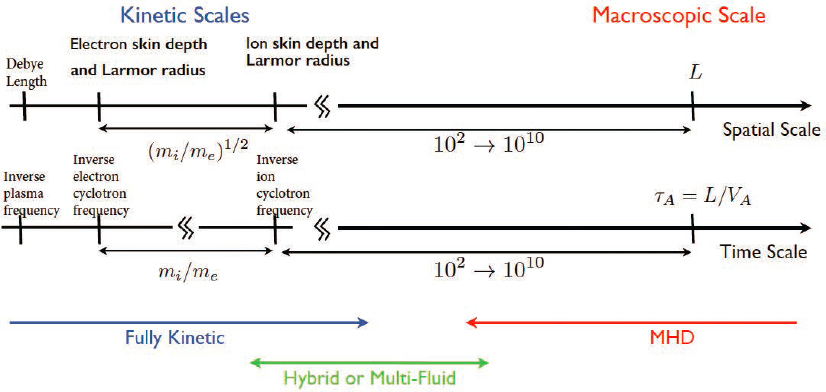
\includegraphics[width=10cm]{immagini/scales.jpg}
		\label{grandezze caratteristiche}
		\caption{lunghezze e tempi caratteristici, fonte: \href{https://www.nationalacademies.org/read/25802/chapter/4\#71}{NationalAcademies.org} }
	\end{figure}
	
\end{approfondimento}

\subsection{Parametro di plasma}

Poiché parliamo di plasmi dobbiamo ricordare di considerare che la frequenza delle collisioni dovrà essere piccola rispetto alla frequenza di plasma:
\[ \frac{\nu^2_{coll.}}{\omega_P^2}\ \sim\ \left(\frac{n^2\, e^8}{m\, T^3} \right) \left(\frac{m}{4\,\pi\, n^2_e} \right)\ \sim\ \frac{e^6 n}{T}\ \ll 1\ \ . \]

Si considera una distanza media fra le particelle $r_n = n^{1/3}$, così che per il rapporto fra energia cinetica e potenziale valga:

\[ \Rightarrow \ \frac{V}{T} \,\sim\, \frac{e^2}{n^{1/3}\, T}\, \sim\, \frac{\nu_{coll.}}{\omega_P}\quad \Rightarrow \quad \frac{V}{T}\ll\ 1\]

La condizione $V\,/\,T\ll\, 1$ è la stessa che si ha in un gas, le collisioni sono molto più alte delle frequenze dinamiche e, nel limite, il rapporto fra la frequenza collisionale e la frequenza dinamica è invece $\gg 1$.

Definiamo la \textbf{sfera di Debye} come la sfera di raggio $\lambda_D$ attorno ad una certa carica qualsiasi. Ci chiediamo in questo paragrafo quante particelle siano contenute in questa sfera.

\[ \text{da definizione:}\quad \quad \lambda_D\ \approx\ \sqrt{\frac{T}{n\, e^2}} \]

Come calcolare il numero di particelle cariche $N_D$ contenute nella sfera?

\[ N_D\, =\, n\,\lambda_D^3 = \sqrt{\frac{n^2\, T^3}{n^3\, e^6}} = \sqrt{\frac{T^3}{n\, e^6}}\, =\, \frac{T^{3/2}}{\sqrt{n}\, e^3}\]

Una prima stima del numero di cariche contenute nella sfera di Debye è $n\, \lambda_D^3$ e - notando che $n\, \lambda_D^3=(T\, /\, V)^{3/2}\ll 1$ - si trova che un plasma rispetta la condizione: $\boxed{N_D\sim n \, \lambda_D^3\gg 1}$.

Si definisce \textbf{parametro di plasma} la grandezza:

\[ \boxed{g\ \equiv\ \frac{\nu_C}{\omega_P}\ =\ \frac{\nu_C}{v_{th}} \frac{v_{th}}{\omega_P} \ =\ \frac{d_e}{\lambda_{mfp}} \ } \]

L'utilità del parametro di plasma sta nel fatto che lega fra di loro le quantità che definiscono scale di grandezza. Si nota che se $\ g\,\gg\, 1\ $ domina il comportamento collettivo ($d_e\gg\lambda_{mfp}$, le collisioni sono ininfluenti), mentre se $\ g\,\ll\, 1\ $ a dominare è l'interazione interparticellare e in questo caso non si ottiene solitamente un plasma.

Considerando $\ r_0 = e^2\, /\, T\ $ ed $\ r_n\, =\, n^{1/3}\ $, il rapporto sarà:
$\ r_n\,/\,r_0\ =\ \displaystyle\frac{n^{1/3}\,T}{e^2}\ =\ \frac{T}{e^2\, n^{1/3}}\ =\ g^{-2/3}\ $, quindi $\ r_n\ =\ r_0 \,g^{-2/3}\ $.

Invece, prendendo $\ \lambda_D\ \sim\ \sqrt{\displaystyle\frac{T}{e^2 \, n_0}}\ $ , dal rapporto $\ \lambda_D\, /\, r_n\ =\ \sqrt{T}\, /\, (e\, \,n^{1/6})\ =\ g^{-1/3}\ $ ricaviamo la relazione $\ \lambda_D\ =\ r_n g^{-1/3}\ $.



%
%
\section{Teorema di connessione (conservazione del flusso)} 

Introduciamo qui alcuni risultati decisamente importanti per la fisica dei plasmi:
\begin{itemize}
	\item \textbf{Teorema di Alfvén}: secondo il \href{https://it.wikipedia.org/wiki/Teorema_di_Alfv%C3%A9n}{teorema di Alfvén} (anche 'legge del congelamento'), in un fluido conduttore con resistività nulla (MHD ideale), le linee di campo 'restano congelate' in un dato volume del fluido, in altri termini il flusso magnetico attraverso ogni superficie S delimitata da un contorno chiuso $C$ in moto in maniera solidale col flusso è costante;
	\item \textbf{Teorema di connessione:} sempre in MHD ideale, se due elementi di plasma ($\vec x_1$, $\vec x_2$) sono inizialmente collegati da una linea di campo magnetico ($d\vec l$), allora rimangono collegati per sempre. Per dirla formalmente: se in $t=0$ si ha che $d\vec l\times \vec B=0$ allora $\forall \, \, t$ successivi valgono sia $\frac{D}{Dt}(d\vec l\times \vec B)=0$ che $d\vec l\times \vec B=0$.
\end{itemize}

Le principali conseguenze di questi teoremi sono che 
\begin{enumerate}
	\item Si conserva la topologia globale
	\item Stati di energia più bassa, ma con topologia diversa, sono proibiti
	\item regioni di plasma non connesse, rimangono per sempre non connesse. 
\end{enumerate} 
è fondamentale per la validità di questi teoremi che valga la legge ideale di Ohm. 
ovvero  è nullo il campo elettrico nel sistema di riferimento dell'elemento fluido \[\vec {E'}=\vec E+\frac{\vec u\times \vec B}{c}=0\] 

\begin{teorema}{conservazione del flusso}{}
	Per capire cosa vuol dire che le linee di campo non si rompono e perché, prendiamo due elementi di fluido infinitamente vicini, $d\vec l$, dopo un tempo dt ciascun punto si muove con la velocità del fluido, $\vec x \rightarrow \vec x + \vec u(\vec x)dt$. 
	
	\[d\vec l+\delta (d\vec l)=d\vec l+ \left[ (\vec u+d\vec u)-\vec u \right] dt \ =\ d\vec l+d\vec udt\implies\delta(d\vec l)=d\vec udt\]  $d\vec u$ è l'incremento del campo di velicità in direzione $d\vec l$\[d\vec u=(d\vec l\cdot \vec \nabla)\vec u\] 
	\[d\vec l+\delta (d\vec l)=d\vec l+ \left[ \vec u(\vec x+d\vec x)-\vec u (\vec x)\right] dt \ =\ d\vec l+(d\vec l\cdot \nabla)\, \vec u\, dt \] 
	
	Capiamo quindi che la variazione nel tempo della distanza fra i due elementi che si muovono è descritto da $\frac{d(\delta\vec l)}{dt}=(\delta \vec l\cdot\vec \nabla)\vec u$. Nota che se $d\vec l$ è lungo una linea di campo allora $d\vec l \times \vec B = 0$, noi ci chiediamo se partendo solo dalle equazioni dell'elettromagnetismo possiamo provare che queste linee di campo non si spezzino.
	Quindi vogliamo calcolare: 
	
	\[\frac{D}{Dt}(\delta\vec l\times\vec B)\ =\ \frac{D\delta\vec l}{Dt}\times \vec B+\delta\vec l\times\frac{D\vec B}{Dt}\]
	
	Consideriamo la legge di faraday e la legge di Ohm ideale:
	\[ \frac{\partial\vec B}{\partial t} = -\nabla \times \vec E\quad \quad \quad \vec E = -\frac{\vec u \times \vec B}{c} \]
	\[\Rightarrow\quad \frac{\partial\vec B}{\partial t}=\vec \nabla\times(\vec u\times\vec B)\]
	
	Seguiamo $\vec B$ attraverso una linea di campo facendo la derivata materiale, questo ci servirà subito l'evoluzione delle linee di campo. Per semplificare l'espressione ci ricordiamo (insomma)  un'identità vettoriale:
	
	\[\frac{D\vec B}{Dt}=\frac{\partial\vec B}{\partial t}+(\vec u\cdot \vec \nabla)\cdot \vec B=(*)\]
	
	\[\vec \nabla\times(\vec u\times\vec B)\ =\ \vec u\,\cancel{( \vec \nabla \cdot \vec B)}-\vec B( \vec \nabla \cdot\vec u) + (\vec B \cdot \vec\nabla)\,\vec u-(\vec u\cdot\vec \nabla)\cdot \vec B\]
	
	\[(*)=\ \vec \nabla\times(\vec u\times\vec B) + (\vec u\cdot \vec \nabla) \vec B\ =\ (\vec B\cdot \vec \nabla)\, \vec u - \vec B\, (\vec \nabla\cdot \vec u)\] 
	
	Sostituendo $\partial\vec B/\partial t$ con l'identità vettoriale, il termine con gradiente della derivata materiale si elide e possiamo cancellare anche  $\vec \nabla\cdot \vec B=0$ per via della seconda equazione di Maxwell.
	
	Allora inserendo questo risultato di $\partial\vec B/\partial t$ assieme a quello prima definito già definito all'inizio di $\frac{d(\delta\vec l)}{dt}=(\delta \vec l\cdot\vec \nabla)\vec u$, si trova infine che l'evoluzione della connesione fra i due elementi fluidi segue: 
	
	\[\frac{d}{dt}(\delta\vec l\times\vec B)=\delta\vec l\times \left[(\vec B\cdot\vec \nabla )\vec u+(\vec B\cdot\vec \nabla )\vec u\right]  +(\delta\vec l\cdot\vec\nabla)\vec u\times\vec B\] 
	
	\vspace{0.5cm}
	
	Se si considera il caso $\delta \vec l\parallel\vec B$, che implica $\delta \vec l\times \vec B = 0$, allora  $\delta\vec l\times(\vec B\cdot\vec \nabla) \vec u=0$ e la formula trovata poco fa va ad annullarsi completamente portando a $\frac{D}{Dt}(\delta \vec l \times \vec B)=0$: per vederlo basta porre $\delta\vec l$ come un riscalamento $\alpha \vec B$:
	
	
	\[\boxed{\frac{d}{dt}(\delta\vec l\times\vec B)=\alpha\vec B\times \left[\cancel{(\vec B\cdot\vec \nabla )\vec u}+(\vec B\cdot\vec \nabla )\vec u\right]  +(\alpha \vec B \cdot\vec\nabla)\vec u\times\vec B \ =\ \dots\ =\ 0}\] 
	
	Si vede abbastanza già così come si annulli tutto grazie alla condizione di parallelismo.
	
	Questo risultato ci porta a osservare che la linea di campo non si rompe finché non avviene la \textit{riconnessione}. Per  violare la legge di Ohm devo avere $\eta\vec J$, sono questi i casi in cui può avvenire la riconnessione (la legge dio Ohm viene violata prima alle scale degli ioni e poi dopo viene violata alle scale degli elettroni).
	
	\[S=\frac{T_r}{T_a}=\frac{T_\text{resistivo}}{T_\text{alfvén}}\] 
	
	La resistività fa capire come in tempi molto più brevi del tempo diffusivo cambia la topologia del campo. 
	
	Flusso magnetico: su una superficie chiusa fa zero, in generale è 
	\[\int_S\vec B\cdot d\vec S=\phi\] 
\end{teorema}

\begin{teorema}{Alfvén}{}
	Finché siamo in MHD ideale vale che:
	\[ \boxed{\ \frac{d\phi}{dt}\ =\ 0\ }\]  
	
	Usando il teorema di Liebnitz per integrare su domini mobili:
	
	\[\frac{d}{dt}\int_{S(t)}\vec B(\vec r,t)\cdot d\vec S=\int_{S(t)}\frac{\partial \vec B}{\partial t}\cdot d\vec S+\oint_{\mathcal{C}(t)}\vec B\cdot (\vec u\times d\vec l)\] 
	
	il primo termine del termine a destra è la variazione locale di flusso dovuta al cambiamento di B nel tempo, il secondo termine invece rappresenta il cambiamento dovuto al fatto che $\mathcal{C}$ si è letteralmente mosso. 
	
	Usiamo anche il teorema di Stokes e che $\vec B\cdot (\vec u\times d\vec l)=-\vec u\times \vec B\cdot d\vec l$
	
	\[\frac{d\Phi}{dt} = \frac{d}{dt}\int_{S(t)}\vec B(\vec r,t)\cdot d\vec S=\int_{S(t)}\bigg(\frac{\partial}{\partial t}\vec B-\nabla\times(\vec u\times \vec B)\bigg)d\vec S\]  
	
	in MHD ideale è valida la legge di Ohm ideale $\frac{\partial\vec B}{\partial t}=\vec \nabla\times(\vec u\times\vec B)$ e quindi 
	
	\[\frac{\partial}{\partial t}\vec B-\nabla\times(\vec u\times \vec B)=0\implies\int_{S(t)}\bigg(\frac{\partial}{\partial t}\vec B-\nabla\times(\vec u\times \vec B)\bigg)d\vec S=0\]  
	
	ed abbiamo così dimostrato il teorema per cui $\boxed{\frac{d\Phi}{dt} = 0}$ .
\end{teorema}
